\section{Optimale Wege}

\subsection{Das Kürzeste-Wege-Problem}

Gegeben sei ein gerichteter, gewichteter Graph $G = (V,E,c)$ mit $c(e) \ge 0$ für alle $(u,v) \in E$. Der Wert $c(e)$ kann zum Beispiel als Länge  (oder allgemein \enquote{Kosten}) interpretiert werden.
Es sind nun ausgehend von einem Startknoten $v_1$ ein kürzester Weg zu jedem anderen Knoten $v_k \in V$ zu finden.

\begin{aussage}
	Es existiert eine Bogenmenge $E_w \subseteq E$ mit $\card{E_w} = \card{V} - 1$, die für jeden Knoten $v_k \neq v_1$ einen kürzesten Weg von $v_1$ zu $v_k$ beinhaltet.
\end{aussage}
\begin{proof}
	Weniger als $\card{V} - 1$ Bögen würden einen Widerspruch zum Zusammenhang liefern. Angenommen es gäbe mehr als $\card{V} - 1$ Bögen. Dann existiert ein Knoten $v \neq v_1$ mit (Eingangs-) Grad $\delta^-(v) \ge 2$, d.h. es gibt zwei optimale Wege von $v$ zu $v_1$. Nur einer dieser Bögen, die in $v$ enden, ist erforderlich, um eine Bogenmenge gemäß Aufgabenstellung zu erhalten.
\end{proof}

\begin{folgerung}
	$E_w$ ist zusammenhängend und kreisfrei, also ein (gerichteter) Spannbaum.
\end{folgerung}

Ein konkretes Verfahren zur Lösung dieses Problems liefert der \person{Dijkstra}-Algorithmus. Dabei werden, ausgehend von einem Startknoten $s = v_1$, bereits bekannte kürzeste Wege durch Hinzufügen weiterer Bögen/Kanten verlängert, um somit kürzeste Wege für bisher unerreichte Knoten zu finden.

Hierfür nutzen wir die Notation: Es sei
\begin{itemize}[nolistsep, topsep=-\parskip]
	\item $M$ die Menge der Knoten, zu denen ein kürzester Weg bekannt ist
	\item $p(v_k) = p(k)$ der Vorgängerknoten von $v_k$ auf dem kürzesten Weg zu $v_k$
	\item $d(v_k) = d(k)$ die Länge des (bisher) kürzesten Weges zu $v_k$
\end{itemize}
Schließlich erhalten wir den folgenden Algorithmus:

\fbox{\textbf{Algorithmus von \person{Dijkstra}:}}
\begin{enumerate}[label=Schritt \arabic*:, leftmargin=*, start=0]
	\item Initialisierung: Setze $M \defeq \menge{s}$, $d(s) = 0$ und initialisiere für $v \neq s$
	\begin{equation*}
		p(v) \defeq \begin{cases}
		s & (s,v) \in E \\ 0 & (s,v) \notin E
		\end{cases} 
		\qquad
		d(v) \defeq \begin{cases}
		c(s,v) & (s,v) \in E \\ +\infty &(s,v) \notin E
		\end{cases}
	\end{equation*}
	\item Bestimme $u \notin M$ mit $d(u) = \min\menge{d(v) : v \notin M}$. Falls $d(u) = +\infty$, dann \texttt{STOP}. Andernfalls setze $M \defeq M \cup \menge{u}$.
	\item Für alle $v \notin M$ mit $(u,v) \in E$: falls $d(v) > d(u) + c(u,v)$ (also ein kürzerer Weg ist gefunden), dann setze $d(v) = d(u) + c(u,v)$ und $p(v) = u$.
	\item Falls $M \neq V$, gehe zu Schritt 1. Sonst \texttt{STOP}.
\end{enumerate}

Offenbar terminiert dieser Algorithmus nach endlich vielen Schritten, da in jeder Iteration entweder ein Element zu $M$ hinzugefügt wird oder der Algorithmus gänzlich abbricht (Schritt 1). Somit wird Schritt 1 höchstens $\mathcal{O}(n)$ mal ausgeführt und bewirkt dabei höchstens $\mathcal{O}(n)$ Durchläufe der in Schritt 2 benötigten Schleife. Bei naiver Implementierung besitzt dieser Algorithmus also eine Komplexität von $\mathcal{O}(\card{V}^2)$, es sind aber auch bessere Abschätzungen (z.B. $\mathcal{O}(\card{E} + \card{V} * \log\card{V})$) möglich.

Sei $d_G(s,v)$ sei die Länge eines kürzesten Weges von $s$ nach $v$ in $G= (V,E,c)$. Offenbar gilt $d(v) \ge d_G(s,v)$ für alle $v \in V$, da der Algorithmus zumindest irgendeinen Weg von $s$ nach $v$ findet oder feststellt, dass es keinen solchen gibt (also $d(v) = \infty$).

\begin{aussage}
	Gilt $c(e) \ge 0$ für alle $e \in E$, so gibt $d(v)$ die Länge eines kürzesten Weges von $s$ nach $v$ an.
\end{aussage}
\begin{proof}
	Sobald ein Knoten $u \in V$ zu $M$ hinzugefügt wird, ändert sich $d(u)$ nicht mehr. Es genügt daher den Zeitpunkt zu betrachten, an dem $u$ zu $M$ hinzugefügt wird.
	\begin{induction}
		\ianfang Als erstes wird (in der Initialisierung) $s$ in $M$ aufgenommen und $d(s) = 0$ gesetzt. Wegen $c(e) \ge 0$ für alle $e \in E$ ist dies die Länge eines kürzesten Weges.
		\ischritt Sei nun $u \neq s$ der \enquote{zeitlich} erste Knoten, für den bei Aufnahme in $M$ die strikte Ungleichung $d(u) > d_G(s,u)$ gilt, d.h. bei $u$ mach der Algorithmus den ersten Fehler. Sei $\gamma$ ein tatsächlich kürzester Weg von $s$ nach $u$. Dieser muss mindestens einen Knoten $y$ enthalten, der (noch) nicht zur Menge $M$ gehört. Wegen $s \in M$ gilt $y \neq s$. Wir zeigen nun, dass $d(y) = d_G(s,y)$ gilt. Offenbar gilt gemäß Induktionsvoraussetzung $d(x) = d_G(s,x)$ für alle Vorgänger $x \in M$ von $y$ auf $\gamma$. Wenn ferner $\gamma$ ein kürzester Weg von $s$ nach $u$ ist, dann enthält $\gamma$ auch einen kürzesten Weg von $s$ nach $y$. Sei $x \in M$ nun der direkte Vorgänger von $y$ auf $\gamma$. Bei der Aufnahme von $x$ in $M$ wurde auch die Kante $(x,y) \in E$ geprüft und folglich $d(y)$ auf den korrekten Wert $d_G(s,y)$ gesetzt. Dann gilt
		\begin{equation*}
			d(u) > d_G(s,u = d_G(s,y) + d_G(y,u) = d(y) + d_G(y,u) \follows d(u) > d(y)
		\end{equation*}
		Also hätte un aktuellen Schritt $u$ nicht in $M$ aufgenommen werde dürfen. Widerspruch.
	\end{induction}
\end{proof}

\begin{beispiel}
	Betrachte folgenden Graphen:
%	(1,2,3)
%	(1,4,2)
%	(1,3,1)
%	(2,4,2)
%	(3,4,1)
%	(4,5,1)
%	(4,6,2)
%	(4,7,1)
%	(5,6,3)
%	(5,8,3)
%	(6,7,1)
%	(7,8,2)

	\begin{minipage}{\dimexpr0.5\linewidth-\fboxrule-\fboxsep}
		\centering
		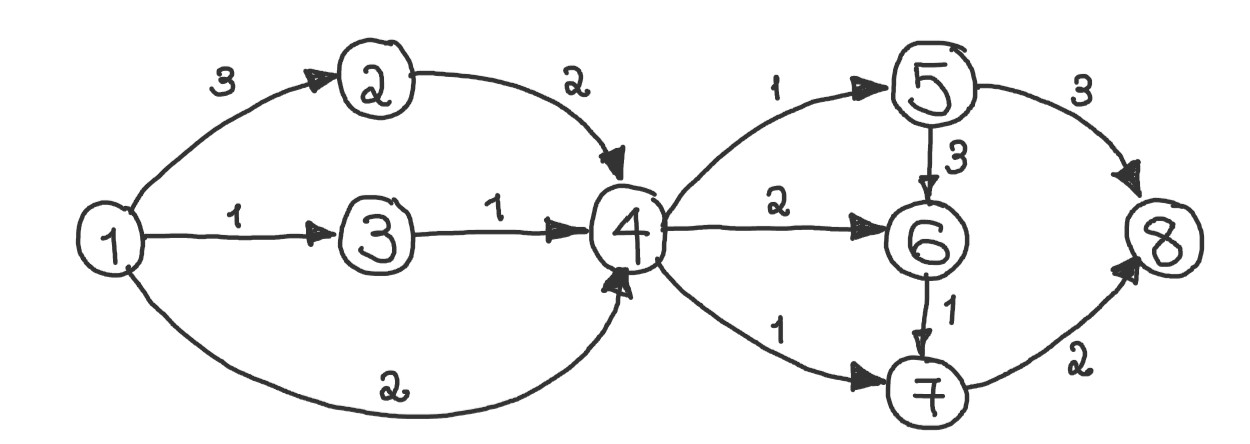
\includegraphics[width=\linewidth]{./optinum_abb/optinum_5_3_bsp5-2.jpg}
	\end{minipage}
	\begin{minipage}{\dimexpr0.5\linewidth-\fboxrule-\fboxsep}
		\begin{tabular}{rccccccccc}
			$p =$ & 0 & $v_1$ & $v_1$ & $v_1$ & $v_4$ & $v_4$ & $v_4$ & \cancel{$v_5$} $v_7$ \\ \hline
			    & $v_1$ & $v_2$ & $v_3$ & $v_4$ & $v_5$ & $v_6$ & $v_7$ & $v_8$ \\ \hline
			$d =$ & \fbox{0} & 3 & \uline{1} & 2 & $\infty$ & $\infty$ & $\infty$ & $\infty$ \\
				&          & 3 &           & \uline{2} & &  & &  \\
				&          & 3 &           &        & 3         & 4 & 3 & \\
				&          &   &           &        & \uline{3} & 4 & 3 & \\
				&          &   &           &        &           & 4 & \uline{3} & 6 \\
				&          &   &           &        &           & \uline{4} &           & 5 \\
		\end{tabular}
	\end{minipage}

	Ein minimaler Weg von $v_1$ nach $v_8$ lautet als
	\begin{equation*}
		v_8 \leftarrow v_7 \leftarrow v_4 \leftarrow v_1
	\end{equation*}
\end{beispiel}


\subsection{Das Längste-Wege-Problem}
\begin{description}
	\item[gegeben:] gerichteter, gewichteter Graph $G = (V,E,c)$ mit beliebiger Funktion $\abb{c}{E}{\R}$
	\item[gesucht:] längste Wege von $s \in V$ zu allen anderen Knoten
	\item[naive Idee:] Dijkstra-Algorithmus für $G' = (V,E,-c)$ --- funktioniert im Allgemeinen nicht, da $-c(e) \ge 0$ nicht erfüllt sein muss
\end{description}

\fbox{\textbf{Algorithmus von \person{Ford}/\person{Moore}:}}
\begin{enumerate}[label=Schritt \arabic*:, leftmargin=*, start=0]
	\item Wähle $s \in V$ als Startknoten und setze $d(s) = 0$, sowie
	\begin{equation*}
		p(v) \defeq \begin{cases}
		s & (s,v) \in E \\ 0 & \text{sonst}
		\end{cases} 
		\qquad
		d(v) \defeq \begin{cases}
		c(s,v) & (s,v) \in E \\ -\infty &\text{sonst}
		\end{cases}
	\end{equation*}
	für alle $s \neq v$. Definiere außerdem $A \defeq \menge{s} \cup \menge{v \in V: (s,v) \in E}$, $B \defeq \emptyset$ und $k \defeq 1$.
	%
	\item Falls $A = \emptyset$ oder $k = \card{V}$, dann \texttt{STOP}.
	\item Für alle $u \in A$ und alle $v \in V$ mit $(u,v) \in E$: falls $d(v) < d(u) + c(u,v)$, dann setze $d(v) = d(u) + c(u,v)$ und $p(v) = u$ sowie $B \defeq B \cup \menge{v}$.
	\item Setze $A = B$, $B = \emptyset$, $k \defeq k+1$ und gehe zu Schritt 1.
\end{enumerate}

Nach Abschluss von Schritt 2 symbolisieren die Mengen $A$ und $B$ diejenigen Knoten, zu denen in der vorherigen bzw. aktuellen Iteration ein längerer Weg gefunden wurde. Das Verfahren von \person{Ford}/\person{Moore} besitzt eine Laufzeit von $\mathcal{O}(\card{V} * \card{E})$ und es kann gezeigt werden:

\begin{aussage}
	Der Algorithmus von \person{Ford}/\person{Moore} ermittelt zu jedem Knoten, der von $s$ erreichbar ist, einen längsten Weg, sofern er mit $A = \emptyset$ terminiert. Andernfalls enthält der Graph Kreise positiver Länge.
\end{aussage}

%Graph: 
%(1,2,1)
%(2,3,2)
%(3,2,3)
%(3,4,4)

Da hierbei die Gewichte $c(e)$ auch negativ sein durften, kann eine modifizierte Variante des Algorithmus zum Auffinden kürzester Wege in beliebigen Graphen genutzt werden.

\subsection{Netzplantechnik}

%\newcommand{\FAZ}{F\!A\!Z}
%\newcommand{\SAZ}{S\!A\!Z}
Längste Wege sind vor allem dann von Interesse, wenn die Wege eines Graphen eine logische Abfolge von Teilprojekten beschreiben, die erfüllt sein müssen, bevor ein neues Teilprojekt starten kann.

\begin{description}
	\item[Formal:]
	\begin{itemize}[nolistsep, topsep=-\parskip]
		\item Teilprojekte $TP_i$ mit Dauer $D_i$ ($i = 1, \dots, N$)
		\item Bedingungen an die Anfangszeiten $\AZ_i$ der Teilprojekte (\begriff{Koppelbedingungen})
	\end{itemize}
	\item[Zielstellung] minimale Gesamtdauer des Projekts (und kritische Teilprojekte)
\end{description}

Wir betrachten zwei Fälle:
\begin{enumerate}[label=(\arabic*), nolistsep]
	\item $\AZ_j \ge \AZ_i + \tau_{ij}$ mit $\tau_{ij} \ge 0$: Teilprojekt $\TP_j$ darf frühestens $\tau_{ij}$ Zeiteinheiten nach Beginn von Teilprojekt $\TP_i$ starten
	\item $\AZ_j \le \AZ_i + \tau_{ji}$ mit $\tau_{ji} \ge 0$: Teilprojekt $\TP_j$ muss spätestens $\tau_{ji}$ Zeiteinheiten nach Beginn von Teilprojekt $\TP_i$ starten
\end{enumerate}

Modellierung als Graph $G = (V,E,c)$:

\begin{itemize}[nolistsep, topsep=-\parskip]
	\item $V = \menge{1, \dots, N}$ entsprechend Teilprojekten
	\item Füge Bögen (gerichtete Kanten) ein gemäß
	\begin{itemize}
		\item $(i,j) \in E$ mit $c(i,j) = \tau_{ij}$ genau dann, wenn Fall (1) vorliegt
		\item $(j,i) \in E$ mit $c(j,i) = \tau_{ji}$ genau dann, wenn Fall (2) vorliegt
	\end{itemize}
\end{itemize}

Die Länge eines Weges von $a \in V$ nach $b \in V$ gibt nun an, wie viele Zeiteinheiten $\AZ_b$ mindestens nach $\AZ_a$ liegen muss. Die maximale Länge aller Wege in $G$ von $a$ nach $b$ sei $\ell(a,b)$ und legt die frühestmögliche Startzeit von $\TP_b$ fest (relativ zur Startzeit von $\TP_a$).

Ohne Einschränkung sei Knoten $1$ der Projektbeginn mit $\AZ_1 = 0$. Ein Algorithmus, der für jedes $TP$ die frühest- und spätestmögliche Anfangszeit $\FAZ_i$ bzw. $\SAZ_i$ bestimmt, kann wie folgt formuliert werden:

\fbox{\textbf{MPM-Algorithmus}}
\begin{enumerate}[label=Schritt \arabic*:, leftmargin=*, start=1]
	\item Ermittle $\FAZ_i$ für alle $i \in V$ gemäß $\FAZ_i = \ell(1,i)$. Definiere $T \defeq \FAZ_N + D_N$ als minimale Projektdauer.
	\item Ermittle $\SAZ_i$ für alle $i \in V$ gemäß $\SAZ_i \defeq \FAZ_N - \ell(i,N)$.
\end{enumerate}

Die Bestimmung von $\ell(1,i)$ kann mit dem \person{Ford}-\person{Moore}-Algorithmus bewerkstelligt werden. Zur Bestimmung von $\ell(i,N)$ kann dieser Algorithmus ebenfalls genutzt werden, wobei dazu $\ell(N,i)$ in einem Graphen gesucht wird, der alle Bögen umorientiert (sodass $N$ der feste Startknoten wird).

\begin{definition}
	Die Zeit $\PZ_i \defeq \SAZ_i - \FAZ_i$ heißt \begriff{Pufferzeit} von $\TP_i$. Ein Teilprojekt $i$ mit $\PZ_i = 0$ heißt \begriff{kritisch}.
\end{definition}

Eine Verzögerung in einem kritischen Teilprojekt beeinflusst die gesamte Projektdauer.

Ein ausführliches Beispiel wird in der Übung besprochen.
